\documentclass{article}
\usepackage{tkz-tab}
\usepackage{amsmath} 
\usepackage{geometry}
\usepackage{indentfirst}
\setlength{\parindent}{0cm} % Retrait du paragraphe
\geometry{
    left=1cm }
\begin{document}
\underline{Tableau de variation de $f(x)$}\\
                   
$f(x)=x^{3} + 3 x$\\
$f'(x)=3 x^{2} + 3$\\

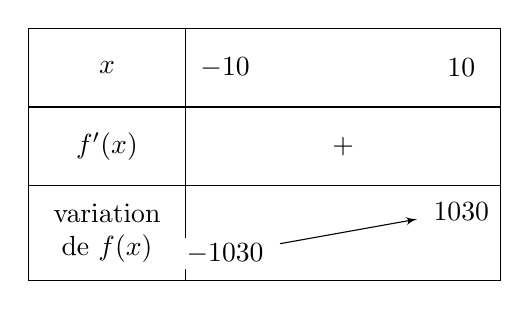
\begin{tikzpicture}
\tkzTabInit[espcl=3]{$x$ / 1 , $f'(x)$ / 1, variation de $f(x)$/1.2}
{$-10$,$10$}
\tkzTabLine{,+}
\tkzTabVar{-/$-1030$,+/$1030$}
\end{tikzpicture}
\end{document}